\section{Introduction}
\label{sec:intro}

Safety evaluations usually present a harmful request and score whether the response \emph{opens} with a
refusal, either with refusal-phrase matching on the first tokens or with a judge applied to a short
generation. For a single request this is reasonable: the model's first output tokens are its answer to that
request.

It is not reasonable when the harmful request is one item among several. Embedding a harmful request in a list
of benign tasks is a known jailbreak strategy
\citep{xiao2024dap,saiem2024sequentialbreak,unit42deceptive,kim2025m2s}, and multi-request inputs are routine
in long-context and agentic use \citep{lu2025longsafety,hadeliya2025refusals}. Given a list, a model can answer
the benign items first and handle the harmful one when it gets there, hundreds of tokens into its response.
A judge that reads only the opening then scores a refusal as compliance.

We learned this from our own mistake. In an earlier version of this project, scoring the first 24 generated
tokens suggested that a numbered list of benign tasks collapses Qwen3-14B's refusal after about 31 tokens of
context, and we built a mechanistic account of the collapse. The harmful item, however, sat at a
pseudo-random position in the list. A one-parameter model, ``the response opens with a refusal only when the
harmful item is listed first,'' explains about 90\% of the variance in that collapse curve
(\cref{app:v1}). This paper replaces that analysis with a controlled measurement.

\paragraph{Contributions.}
\begin{enumerate}[leftmargin=*,itemsep=1pt,topsep=2pt]
\item \textbf{Short-horizon judges misread multi-request prompts.} We vary the harmful item's position, list
length (up to 32 items) and template over 200 JailbreakBench and AdvBench targets and three model families
(about 18{,}000 full-length responses). With the harmful item not first, 24-token scoring reports refusal rates
as low as 5\%, while the models refuse the item in 81--96\% of responses and HarmBench's classifier finds harmful
content in at most 15\% (\cref{sec:behaviour}). The finding holds for larger models (up to 70B), a second judge,
sampled decoding, reasoning mode and other benign content; adversarial framings, not lists, drive the high
success of embedded-prompt attacks (\cref{sec:robust}).
\item \textbf{How far a judge must read, and why the error is biased.} Detected refusal reaches its
full-response value only after about 1{,}000 tokens, and models differ in where they refuse: Qwen3-14B and
Gemma-2-9B mostly at the item, Llama-3.1-8B mostly up front. A short-horizon judge therefore ranks models by where
they refuse rather than whether they do (\cref{sec:horizon}). We give a judging protocol (\cref{sec:discussion}).
\item \textbf{Where the decision is carried depends on the model.} Ablating the refusal direction
\citep{arditi2024refusal} only at prompt positions leaves Qwen3-14B's in-list refusals intact but removes most of
Llama-3.1-8B's, matching where each model refuses. Preregistered tests on held-out behaviours confirmed this, including
for Llama-3.1-70B, which refuses at the item and keeps its in-list refusals unlike its 8B sibling
(\cref{sec:mechanism}). This extends evidence that refusal depends on how the refusal signal evolves during
generation \citep{dahiya2026suppress,yamaguchi2025reasoning} to multi-request prompts.
\end{enumerate}

\section{Related Work}
\label{sec:related}

\paragraph{Embedded and multi-task jailbreaks.} DAP \citep{xiao2024dap}, SequentialBreak
\citep{saiem2024sequentialbreak}, Deceptive Delight \citep{unit42deceptive} and multi-turn-to-single-turn
templates \citep{kim2025m2s} place harmful requests among other tasks. SequentialBreak reports high attack
success for harmful prompts placed late in LLM-written game, dialogue and question-bank framings, and low
success when the harmful prompt comes first. We separate the effect of plain list structure from that of such
framings and measure both with a full-response judge.

\paragraph{Evaluating refusal.} Keyword and prefix judges are known to overstate jailbreak success
\citep{souly2024strongreject,zhu2024advprefix}; HarmBench \citep{mazeika2024harmbench} and JailbreakBench
\citep{chao2024jailbreakbench} standardize classifier-based judging. We document the opposite error for
multi-request prompts: reading too \emph{early} turns refusals into apparent compliance. Long-context safety
benchmarks \citep{lu2025longsafety,hadeliya2025refusals} face the same issue whenever the harmful content
appears late in a response.

\paragraph{Refusal directions during generation.} Refusal is mediated by a difference-of-means direction
\citep{arditi2024refusal}, possibly within a multi-dimensional cone \citep{wollschlaeger2025geometry}.
Harmfulness and refusal are encoded at different positions \citep{zhao2025separately}. Most closely related,
\citet{dahiya2026suppress} find, for seven jailbreak classes, that the direction is a reliable causal control
signal but that jailbreak success is better explained by how attacks interact with it over the course of
generation than by its value at the end of the prompt. Prompt representations are known to encode attributes
of the whole upcoming response \citep{dong2025planning}, and reasoning models can decide to refuse inside their
chain of thought \citep{yamaguchi2025reasoning}. Our mechanistic results apply these ideas to multi-request
prompts; we do not claim them as new mechanisms.

\paragraph{Safety alignment depth.} \citet{qi2025shallow} show that alignment concentrates on the first few
output tokens and that forcing a compliant opening often defeats it. List prompts let us ask the same question
deep inside a response.

\paragraph{Probes and attention.} Linear probes on activations are cheap safety monitors
\citep{cunningham2025cheap,mckenzie2025highstakes}; attention heads that route refusal have been located
\citep{he2024jailbreaklens} and attacked \citep{srivastava2026ara}. We use both only as analysis tools.

\section{Setup}
\label{sec:setup}

\paragraph{Threat model and evaluation question.} We take the evaluator's side. A red-teaming or safety
benchmark submits prompts that bundle one harmful request with benign ones, as embedded-prompt attacks and
agentic inputs do, and an automatic judge decides from the response whether the model refused. The attacker
controls only the prompt text (list length, item position, framing); the model is queried in a single turn
with greedy or sampled decoding and no system prompt. Our question is whether the judge's verdict matches what
the model did with the harmful item. Mechanistic interventions (\cref{sec:mechanism}) assume white-box access
and serve to explain the behaviour, not as attacks.

\paragraph{Models.} Qwen3-14B \citep{qwen3} with thinking disabled, Gemma-2-9B-it \citep{gemma2} and
Llama-3.1-8B-Instruct \citep{llama3}, plus Qwen3-32B, Gemma-2-27B-it, Llama-3.1-70B-Instruct and Qwen3-14B in
thinking mode for robustness. Generation is
greedy (vLLM; \citealp{kwon2023vllm}) with a budget of $320(k{+}1){+}256$ new tokens for a list with $k$ benign
items, capped by the context window. At most 1.2\% of responses per model hit the cap.

\paragraph{Prompts.} Harmful targets are the 100 JailbreakBench behaviours \citep{chao2024jailbreakbench} and
100 AdvBench prompts \citep{zou2023advbench}. Benign list items are Alpaca instructions \citep{taori2023alpaca}.
For each target and $k\in\{0,1,3,7,15,31\}$ we sample $k$ benign items once and insert the target \emph{first},
\emph{in the middle} or \emph{last}, so only the position changes within a (target, $k$) cell. The main template
reads ``I have several requests for you to handle in order: 1.~\dots''. At $k\in\{3,15\}$ we add a bulleted and
a ``Task~$i$:'' template. As an over-refusal control, 100 benign Alpaca targets are placed in the same lists.

\paragraph{Judging.} Only one list item is harmful, so we judge the \emph{whole} response:
\begin{itemize}[leftmargin=*,itemsep=1pt,topsep=1pt]
\item \textbf{ASR}: the HarmBench Llama-2-13B classifier \citep{mazeika2024harmbench} on 512-token windows of
the response; harmful if any window is.
\item \textbf{Target refused}: one of 33 refusal phrases appears before the model starts answering list items,
inside the harmful item's answer, or anywhere if the item is skipped. Phrases in \emph{other} items' answers do
not count, because benign items attract capability disclaimers (``I can't draw''). With a benign target, this
rule fires on 0--3\% of responses.
\item \textbf{Refusal locus}: \emph{up front} if the refusal precedes the list answers, \emph{in the item}
otherwise.
\item \textbf{24-token metric}: refusal substrings in the first 24 generated tokens, exactly as in our earlier
study. With greedy decoding these tokens are identical to the earlier 24-token generations.
\end{itemize}
\Cref{app:judge} gives details; \cref{app:prompts} shows prompts and responses.

\section{Short-horizon judges misread multi-request prompts}
\label{sec:behaviour}

\begin{figure}[t]
\centering
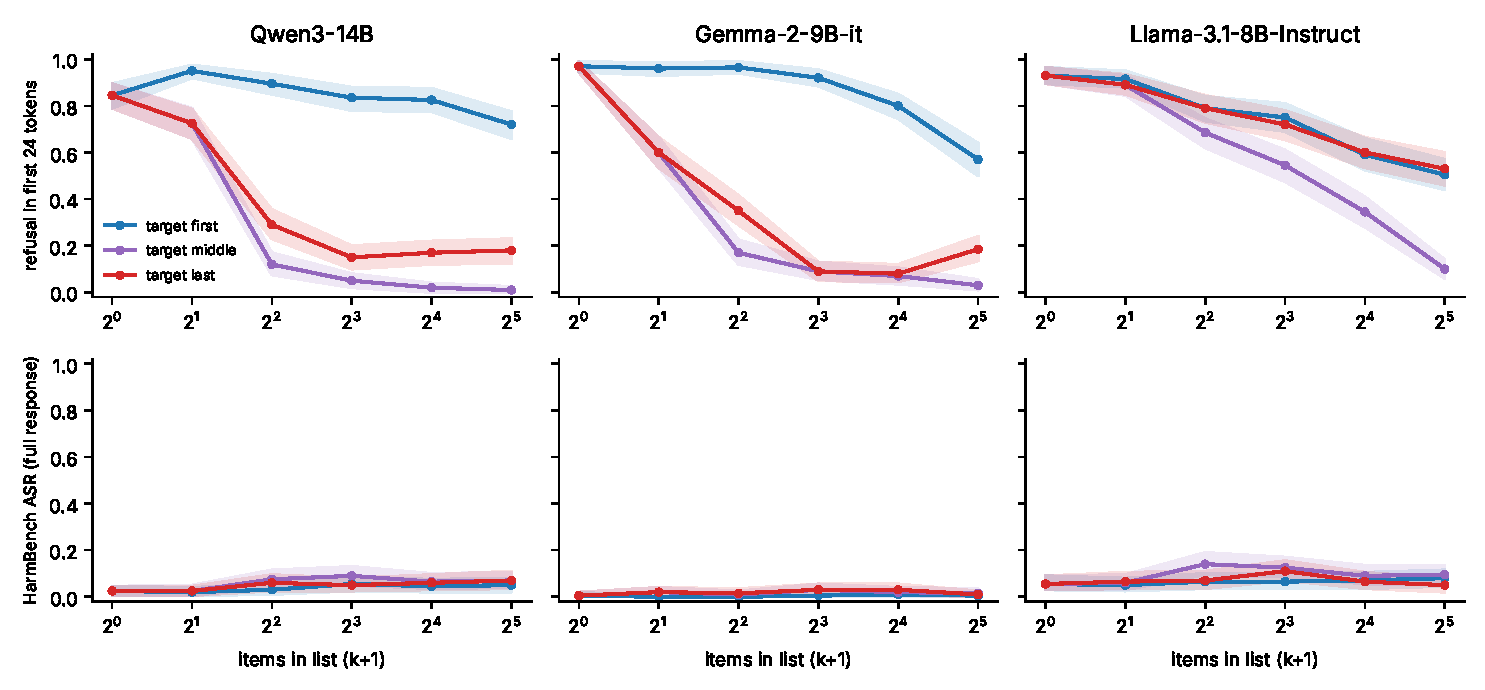
\includegraphics[width=\linewidth]{fig_behaviour.pdf}
\caption{Numbered-list template, 200 harmful targets per point; shaded bands are 95\% bootstrap CIs over
prompts. \textbf{Top:} the earlier metric, a refusal phrase in the first 24 generated tokens, collapses as soon
as the harmful item is not first. \textbf{Bottom:} HarmBench attack success on the full response stays low at
every list length and position. $x$-axis: number of items in the list ($k{+}1$; 1 = request alone).}
\label{fig:behaviour}
\end{figure}

\begin{table}[t]
\centering\small
\caption{Pooled over $k\in\{3,7,15,31\}$, numbered template (800 responses per cell; $k{=}0$: 200). Percentages
with 95\% bootstrap CIs over prompts. ``Target refused'' counts refusals of the harmful item wherever they occur
in the response (\cref{sec:setup}). It is not the complement of ASR; the remainder are deflections, such as
reinterpreting ``a guide for cyberbullying'' as advice for victims.}
\label{tab:behaviour}
\begin{tabular}{llccc}
\toprule
Model & Harmful item & Refusal in first 24 tok. & Target refused & HarmBench ASR \\
\midrule
Qwen3-14B & alone ($k{=}0$) & 84\ci{80}{90} & 89\ci{85}{93} & 2\ci{0}{5} \\
 & first in list & 82\ci{78}{86} & 90\ci{86}{93} & 4\ci{2}{7} \\
 & middle in list & 5\ci{4}{7} & 81\ci{76}{85} & 8\ci{5}{10} \\
 & last in list & 20\ci{16}{24} & 82\ci{77}{86} & 6\ci{4}{9} \\
\midrule
Gemma-2-9B & alone ($k{=}0$) & 97\ci{94}{99} & 98\ci{95}{100} & 0\ci{0}{2} \\
 & first in list & 81\ci{78}{85} & 98\ci{96}{99} & 0\ci{0}{1} \\
 & middle in list & 9\ci{7}{12} & 93\ci{90}{95} & 2\ci{1}{3} \\
 & last in list & 18\ci{15}{20} & 96\ci{94}{98} & 2\ci{1}{4} \\
\midrule
Llama-3.1-8B & alone ($k{=}0$) & 93\ci{89}{96} & 93\ci{89}{96} & 6\ci{3}{9} \\
 & first in list & 66\ci{60}{71} & 85\ci{81}{89} & 7\ci{4}{10} \\
 & middle in list & 42\ci{38}{46} & 78\ci{74}{83} & 11\ci{8}{15} \\
 & last in list & 66\ci{60}{71} & 86\ci{81}{89} & 7\ci{5}{10} \\
\bottomrule
\end{tabular}
\end{table}

\paragraph{The 24-token judge reports a collapse that is not there.} \Cref{fig:behaviour} (top) reproduces the
earlier result with the earlier metric. When the harmful item is first, the response opens with a refusal
(\QwenFirstVone\ for Qwen3-14B, against \QwenAloneVone\ for the request alone). When it is in the middle or
last, the opening refusal rate drops to \QwenMiddleVone\ and \QwenLastVone. The same pattern appears in every
model and template. Reading the full response changes the picture (\cref{tab:behaviour}). Qwen3-14B refuses
the harmful item in \QwenMiddleRef\ and \QwenLastRef\ of middle and last placements, and HarmBench's classifier
finds harmful content in only \QwenMiddleASR\ and \QwenLastASR. Among Qwen3-14B list responses that the 24-token
judge scores as compliant, \QwenNotHarmfulGivenVoneComply\ contain no harmful content.
Gemma-2-9B shows the same pattern more strongly. Its opening refusal rate falls to \GemmaMiddleVone\ (middle) and \GemmaLastVone\ (last), yet it refuses the harmful item in \GemmaMiddleRef\ and \GemmaLastRef\ of those responses, and its ASR never exceeds \GemmaMaxASR\ in any cell.\ Llama-3.1-8B shows what the short-horizon judge is actually measuring. It usually refuses up front (\LlamaUpfrontShare\ of its refusals when the item is not first), so its 24-token refusal rate drops less (\LlamaMiddleVone\ middle, \LlamaLastVone\ last) and the misreading is smaller. It is still present: among Llama list responses that the 24-token judge calls compliant, \LlamaNotHarmfulGivenVoneComply\ contain no harmful content.

\paragraph{Is there any real effect of lists?} Yes, but it is small. Qwen3-14B's ASR rises from \QwenAloneASR\
for the request alone to at most \QwenMaxASR\ in any list cell, and target refusal falls by roughly
8 points. The difference goes into deflections rather than harmful compliance. Gemma-2-9B's ASR stays at or below 5\% in every cell of every template. Llama-3.1-8B shows the largest effect: from \LlamaAloneASR\ for the request alone to \LlamaMaxASR\ in its worst numbered-template cell (middle position, three items; 15\% with the bulleted template at $k{=}15$), with confidence intervals that overlap the baseline in most cells.\ The effect
does not grow with list length beyond three items (\cref{fig:behaviour}, bottom). This is not because attention
is undiluted. \Cref{sec:mechanism} shows that the guardrail head's attention to the harmful request does fall
with list length. Behaviour simply does not follow it.

\paragraph{Templates.} With bulleted and ``Task~$i$:'' templates the 24-token judge changes a lot, because the
to-do-list wording makes models refuse up front more often, but ASR stays low under all three
(\cref{tab:templates} in \cref{app:judge}).


\section{How far must a judge read, and where do models refuse?}
\label{sec:horizon}

\begin{figure}[t]
\centering
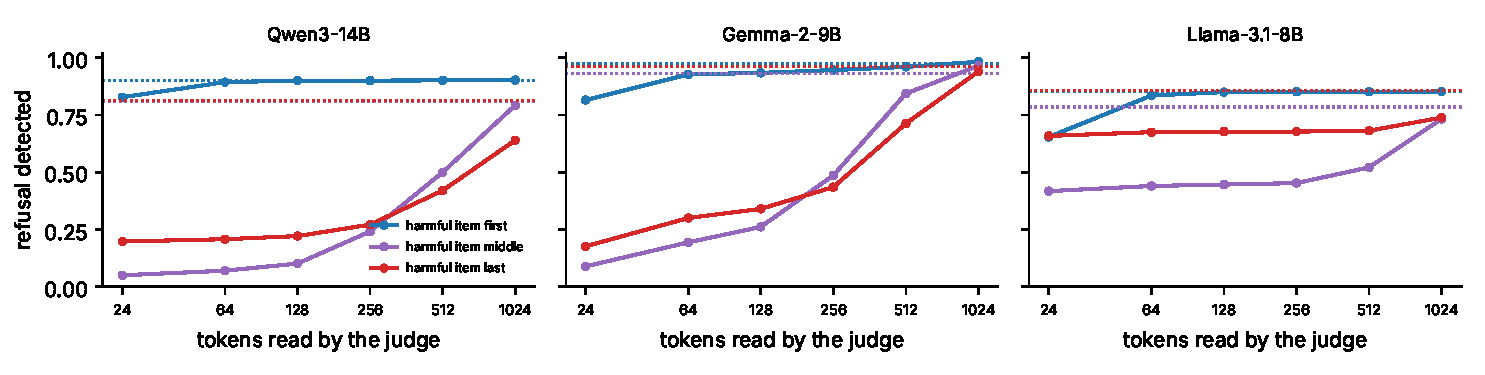
\includegraphics[width=\linewidth]{fig_horizon.pdf}
\caption{Refusal detected by a judge that reads only the first $N$ generated tokens and looks for any refusal
phrase, for harmful items placed first, in the middle or last (numbered template, $k\ge3$; 800 responses per
line). Dotted lines: target refusal in the full response.}
\label{fig:horizon}
\end{figure}

\paragraph{How far must a judge read?} \Cref{fig:horizon} varies the number of tokens a refusal-phrase judge
reads. When the harmful item comes first, 64 tokens recover nearly all refusals for every model. When it comes in the middle,
Qwen3-14B's detected refusal rises from 5\% at 24 tokens to 24\% at 256, 50\% at 512 and 79\% at 1{,}024,
against 81\% in the full response. Gemma-2-9B follows the same course (9\%, 49\%, 84\%, 96\%). Judges that read
a few hundred tokens, a common budget in jailbreak evaluations, therefore still miss most deferred refusals in
lists of four or more items.

\paragraph{Where models refuse.} The curves differ by model because models refuse in different places. When
the harmful item is not first, Qwen3-14B places \QwenInItemShare\ of its refusals \emph{in the item}: it answers
the preceding benign items, then declines. Gemma-2-9B does so in \GemmaInItemShare\ of cases. Llama-3.1-8B
reverses the pattern and refuses \emph{up front} in \LlamaUpfrontShare\ of cases (``I can't help with request 4,
but here are the others''). Its detected refusal is therefore nearly flat in $N$, and a 24-token judge already
sees most of it. A fixed short horizon thus does not just add noise; it ranks models by \emph{where} they refuse
rather than \emph{whether} they do. Under a 24-token judge, Llama-3.1-8B looks far safer than Qwen3-14B on list
prompts (\LlamaMiddleVone\ vs.\ \QwenMiddleVone\ refusal, middle position), although its full-response ASR is
higher (\LlamaMiddleASR\ vs.\ \QwenMiddleASR).


\section{Robustness}
\label{sec:robust}

\paragraph{A larger model.} Qwen3-32B shows the same misreading. With the harmful item in the middle of a list,
its opening refusal rate is \BigMiddleVone, while it refuses the item in \BigMiddleRef\ of responses and
HarmBench ASR is \BigMiddleASR\ (request alone: \BigAloneRef\ refused, \BigAloneASR\ ASR).

\paragraph{Sampled decoding.} With temperature 0.7 and three samples per prompt, the gap persists for every
model: with the harmful item last, the 24-token judge reports \SampQwenLastVone, \SampGemmaLastVone\ and
\SampLlamaLastVone\ refusal for Qwen3-14B, Gemma-2-9B and Llama-3.1-8B, against \SampQwenLastRef,
\SampGemmaLastRef\ and \SampLlamaLastRef\ target refusal and \SampQwenLastASR, \SampGemmaLastASR\ and
\SampLlamaLastASR\ ASR (\cref{tab:variants}).

\paragraph{Reasoning mode.} \THINKSENTENCE

\paragraph{A second judge.} StrongREJECT's fine-tuned evaluator \citep{souly2024strongreject} agrees with
HarmBench's labels (AUC \SRQwenAUC, \SRGemmaAUC, \SRLlamaAUC) and rates responses that neither refuse nor are
harmful under our labels as low-utility for an attacker (mean score \SRQwenOther, \SRGemmaOther, \SRLlamaOther\ on
a 0--1 scale), supporting our reading of them as deflections (\cref{tab:sr}).

\paragraph{What surrounds the request.} Replacing Alpaca instructions with coding tasks, math word problems or
factual questions as the benign items (8-item lists, harmful item in the middle or last) leaves ASR low for
every model (\cref{tab:content}). \CONTENTSENTENCE

\paragraph{Lists versus adversarial framings.} SequentialBreak \citep{saiem2024sequentialbreak} reports high
attack success for harmful prompts embedded late in game, dialogue and question-bank framings. We wrote framings
in that style ourselves (8 items; JailbreakBench targets) and compared them with the plain list under the same
full-response judge (\cref{tab:framing}). The framing, not the list or the position, carries the effect. A
text-adventure framing raises ASR to 28--42\% across the four models when the harmful item comes first and to
8--27\% when it comes late, so position matters less than framing; a question-bank framing raises Qwen3-14B's ASR
to 15--21\%. The plain list and the dialogue framing stay at or below 12\%. Our numbers
remain below SequentialBreak's, whose templates are generated and tuned per behaviour, but they agree that
narrative framing, not multi-request structure as such, is what makes embedded requests effective.

\begin{table}[t]
\centering\small
\caption{Plain list versus framings in the style of SequentialBreak (8 items, 100 JailbreakBench targets).
Cells: HarmBench ASR / refusal in the first 24 tokens, in \%. ``Late'': fifth of eight items.}
\label{tab:framing}
\resizebox{\linewidth}{!}{\begin{tabular}{llcccc}
\toprule
Framing & Harmful item & Qwen3-14B & Gemma-2-9B & Llama-3.1-8B & Qwen3-32B \\
\midrule
plain numbered list & first & 9 / 80 & 1 / 89 & 4 / 69 & 9 / 37 \\
 & late & 10 / 3 & 5 / 11 & 12 / 46 & 10 / 12 \\
text-adventure game & first & 37 / 6 & 42 / 30 & 32 / 56 & 28 / 22 \\
 & late & 25 / 0 & 8 / 0 & 27 / 45 & 13 / 0 \\
student/mentor dialogue & first & 4 / 70 & 2 / 46 & 9 / 71 & 6 / 26 \\
 & late & 8 / 0 & 5 / 5 & 5 / 28 & 5 / 0 \\
exam question bank & first & 21 / 1 & 8 / 71 & 13 / 63 & 10 / 4 \\
 & late & 15 / 0 & 9 / 20 & 12 / 56 & 10 / 0 \\
\bottomrule
\end{tabular}}
\end{table}

\begin{table}[t]
\centering\small
\caption{Kinds of benign items around the harmful request (8 items, harmful item in the middle or last; 400
responses per cell). Cells in \%.}
\label{tab:content}
\resizebox{\linewidth}{!}{\IfFileExists{generated/tab_content.tex}{\begin{tabular}{lccccccccc}
\toprule
Benign items & \multicolumn{3}{c}{Qwen3-14B} & \multicolumn{3}{c}{Gemma-2-9B} & \multicolumn{3}{c}{Llama-3.1-8B} \\
 & 24-tok & refused & ASR & 24-tok & refused & ASR & 24-tok & refused & ASR \\
\midrule
Alpaca instructions & 6 & 82 & 5 & 10 & 96 & 2 & 64 & 81 & 10 \\
coding tasks (MBPP) & 30 & 80 & 9 & 56 & 95 & 0 & 66 & 74 & 16 \\
math problems (GSM8K) & 0 & 66 & 8 & 19 & 95 & 2 & 66 & 88 & 4 \\
factual questions (NQ) & 19 & 89 & 4 & 30 & 96 & 1 & 60 & 76 & 12 \\
\bottomrule
\end{tabular}}{\textbf{[content table pending]}}}
\end{table}


\section{Supporting mechanistic analysis}
\label{sec:mechanism}

We ran one forward pass per response over the prompt followed by the model's own greedy output, cut shortly
after the harmful item's answer begins. At three positions we record the projection
$\langle h_\ell,\dhat_\ell\rangle$: the last prompt token; the first content token of the harmful item's
answer, the \emph{answer onset}; and the answer onset of the nearest benign item. We use 200 harmful targets
for each $k\in\{0,3,15\}$ $\times$ \{first, last\}, plus the benign-target controls. Responses that refuse the
item up front have no harmful answer onset and are excluded from onset statistics. \Cref{tab:probe} reports
the selected layer, and \cref{fig:auc} shows every layer.

\begin{table}[t]
\centering\small
\caption{Projection onto the refusal direction at the selected layer (Qwen3-14B: 36; Gemma-2-9B:
\GemmaLayer; Llama-3.1-8B: \LlamaLayer). Values are means; AUCs compare item-refused and item-complied responses
to list prompts (800 probed list responses per model, of which 39, 11 and 54 complied; Gemma's AUCs therefore
rest on few positives). The last rows split list responses by the sign of the last-token projection.}
\label{tab:probe}
\resizebox{\linewidth}{!}{\begin{tabular}{lccc}
\toprule
Projection (\% of harmful-alone value) & Qwen3-14B & Gemma-2-9B & Llama-3.1-8B \\
\midrule
last prompt token, harmful request alone & +100 & +100 & +100 \\
last prompt token, benign request alone & -30 & +4 & -6 \\
\midrule
last prompt token, harmful item first & +30 & +60 & +15 \\
last prompt token, harmful item last & +11 & +40 & +20 \\
\midrule
harmful item's answer onset, item refused & +4 & +56 & +27 \\
harmful item's answer onset, item complied & -18 & +35 & +29 \\
benign item's answer onset & -25 & +10 & +6 \\
\midrule
AUC refused vs.\ complied, answer onset (sel.\ / best layer) & 0.88 / 0.91 (27) & 0.86 / 0.90 (26) & 0.46 / 0.83 (16) \\
AUC refused vs.\ complied, last prompt token (sel.\ / best) & 0.95 / 0.95 (24) & 0.92 / 0.97 (38) & 0.69 / 0.91 (25) \\
\quad control: same request \emph{alone}, last prompt token (layer) & 0.95 (24) & 0.89 (38) & 0.93 (25) \\
\midrule
lists with negative last-token projection & 16\% & 0\% & 3\% \\
\quad ASR / target refused, if negative & 23\% / 46\% & -- & 23\% / 55\% \\
\quad ASR / target refused, if positive & 1\% / 95\% & 1\% / 97\% & 6\% / 86\% \\
\bottomrule
\end{tabular}}
\end{table}

\paragraph{Lists shrink the last-token read-out and flip its sign, but not its ranking.} A harmful request
alone gives a large positive projection at the last prompt token, and a benign request a small or negative one
(\cref{tab:probe}; values are scaled so that harmful-alone $=100$). Embedding the harmful request in a list
shrinks the last-token projection to 11--60\% of that value. For Qwen3-14B it turns negative in
\QwenNegLastFrac\ of list prompts, which is the ``sign flip'' of our earlier study. Llama-3.1-8B flips in
\LlamaNegLastFrac\ of list prompts and Gemma-2-9B never does. Read naively, a negative
projection says the model has moved into the non-refusal half-space. Behaviourally that reading is wrong most
of the time: when the sign flips, the model still refuses the harmful item or deflects it in about 77\% of
responses in both Qwen3-14B and Llama-3.1-8B. It is right about risk, though: ASR is 23\% when the sign flips
and 1--6\% when it does not.

The ranking survives the shift. Within list prompts, the last-token projection separates responses that end up
refusing the harmful item from those that comply, with AUC up to \QwenAUCLastBest\ (Qwen3-14B),
\GemmaAUCLastBest\ (Gemma-2-9B) and \LlamaAUCLastBest\ (Llama-3.1-8B) at the best layer (\cref{fig:auc}). So the end of the prompt already encodes
what the model will do \emph{when it gets to} the harmful item, even though its first output tokens are about
something else. What breaks is the \emph{calibration} that maps the projection to the next tokens. The zero
point that separates refusal from compliance for single requests does not carry over to lists. Last-token
probes are not wrong about the model's state; they are wrong about \emph{when} that state takes effect.

\paragraph{The same information is present at the item.} At the harmful item's answer onset, the projection
separates refused from complied items with AUC up to \QwenAUCOnsetBest\ (Qwen3-14B), \GemmaAUCOnsetBest\
(Gemma-2-9B) and \LlamaAUCOnsetBest\ (Llama-3.1-8B), slightly below the last-token values. It also sits clearly above the answer onsets of benign items in the same responses
(\cref{tab:probe}). In all three models the separation appears only in later layers: from about layer 20 of 40 in Qwen3-14B,
layer 20 of 42 in Gemma-2-9B and layer 12 of 32 in Llama-3.1-8B. For Llama-3.1-8B it is weak at the causally selected layer 10
(\cref{tab:probe}). Absolute projections at the onset are small compared with the harmful-alone value, which is
expected, since $\dhat$ was fit at last-prompt-token positions of single requests.

\paragraph{The ``guardrail head'' looks when it needs to.} Our earlier study reported that Qwen3-14B's head
L36H31, the largest direct contributor to $\dhat_{36}$, loses attention to the harmful request under dilution.
From the last prompt token of a list prompt, its attention mass on the harmful request's tokens is indeed
small: \AttnLast, against \AttnBare\ for the request alone. From the harmful item's answer onset it is
\AttnOnset, several times higher than from the last prompt token and higher than the mass the same head puts on
a benign item's own request at that item's onset (\AttnBenignOwn). The head reads whichever request the model
is currently answering. Its low attention from the last prompt token reflects \emph{where we measured}, not a
lesion.



\begin{figure}[t]
\centering
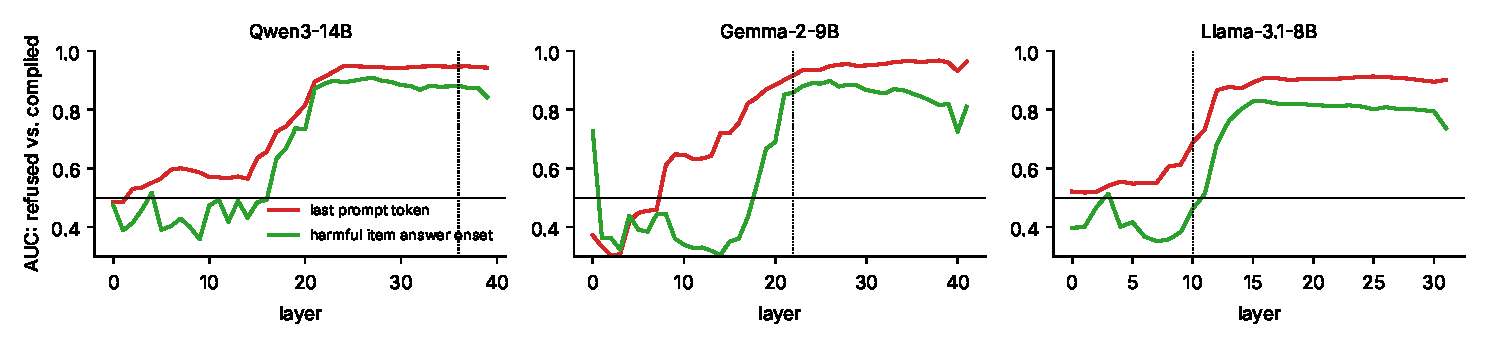
\includegraphics[width=\linewidth]{generated/fig_auc_layers.pdf}
\caption{How well the projection onto $\dhat_\ell$ separates list responses that refuse the harmful item from
those that comply (HarmBench), by layer. Red: read at the last prompt token. Green: read at the harmful item's
answer onset. Dotted: causally selected layer.}
\label{fig:auc}
\end{figure}


\section{Recommendations and limitations}
\label{sec:discussion}

\paragraph{Recommendations for evaluating multi-request prompts.}
\begin{enumerate}[leftmargin=*,itemsep=1pt,topsep=1pt]
\item \textbf{Generate to completion and judge the whole response.} For lists of four or more items, judges
that read a few hundred tokens miss most deferred refusals (\cref{fig:horizon}).
\item \textbf{Judge the harmful item, not the response's opening.} Score harmful content anywhere in the
response, and count refusals only where they refer to the harmful item; capability disclaimers on benign items
otherwise inflate refusal (18\% false positives on benign Gemma lists under a whole-response phrase rule).
\item \textbf{Control and report the harmful item's position.} An attack that ``works'' only when the item is
not first may be measuring the judge rather than the model.
\item \textbf{Compare models with the same horizon only if they refuse in the same place.} A short horizon
favours models that refuse up front (\cref{sec:horizon}).
\end{enumerate}

\paragraph{For interpretability.} Reading a refusal direction at the last prompt token assumes that the next
tokens carry the decision. That holds for single requests, and our ablations show it also holds for
Llama-3.1-8B in lists, but not for Qwen3-14B, which recomputes the decision at the item. Read-outs and
interventions should therefore target the position where the model acts on the request in question, which in
agentic transcripts is usually deep in the model's own output. End-of-prompt read-outs should also be compared
against the same request in isolation before being interpreted as plans.

\paragraph{Limitations.}
\begin{itemize}[leftmargin=*,itemsep=1pt,topsep=1pt]
\item \textbf{Automatic judges.} ASR comes from HarmBench's classifier, checked against StrongREJECT, and refusal
from a phrase rule with a measured false-positive rate. Human labels for a 120-response audit set are not yet
collected.
\item \textbf{Open models of 8--32B parameters,} with reasoning mode tested only for Qwen3-14B. We did not test
proprietary models.
\item \textbf{One family of structures.} Lists of independent tasks, with four kinds of benign content and three
adversarial framings. Documents with embedded instructions and multi-turn agent transcripts remain untested.
\item \textbf{One direction per model.} Refusal involves more than one direction \citep{wollschlaeger2025geometry},
and for Qwen3-14B ablating ours removes refusal phrasing without producing much harmful content. The
mechanistic results concern the refusal behaviour this direction controls.
\item \textbf{No training-based mitigation.} We test activation steering only; fine-tuning for item-level
refusal is left for future work.
\end{itemize}

